\begin{frame}[t]{Background}

\begin{columns}
\begin{column}{0.6\textwidth}
    \begin{itemize}
        \item 
    \end{itemize}
\end{column}
\begin{column}{0.4\textwidth}
\begin{figure}[h]
  \centering
  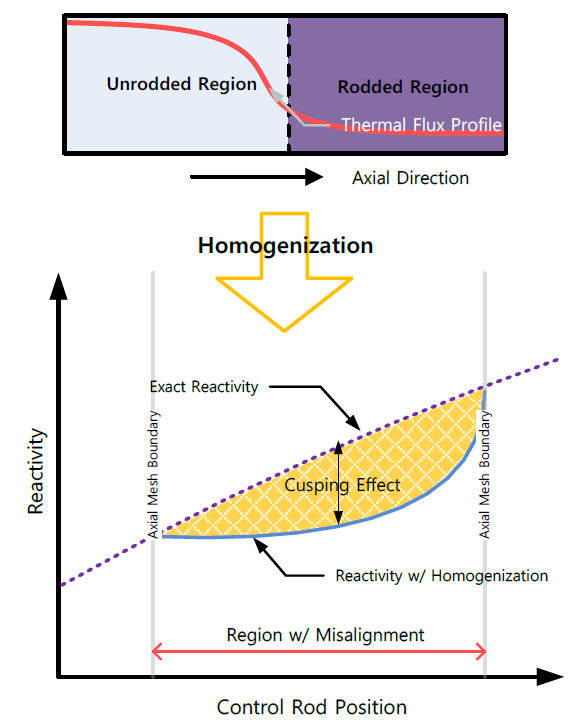
\includegraphics[width=\textwidth]{cusping_effect_Joo.png}
\end{figure} 
\end{column}
\end{columns}
    
\end{frame}

%%%%%%%%%%%%%%%%%%%%%%%%%%%%%%%%%%%%%%%%%%%%%%%%%%%%%%%%%%%%%%%%%%%%%%%%%%%%%%%%%

\begin{frame}[t]{2D/1D Decusping Methods}
    
    \begin{itemize}
        \item Nodal Methods
        \begin{itemize}
            \item 
        \end{itemize}
        \item 2D/1D
        \begin{itemize}
            \item 
        \end{itemize}
        \item
    \end{itemize}
    
\end{frame}

%%%%%%%%%%%%%%%%%%%%%%%%%%%%%%%%%%%%%%%%%%%%%%%%%%%%%%%%%%%%%%%%%%%%%%%%%%%%%%%%%

\begin{frame}[t]{Sub-Plane Decusping}
    
\begin{itemize}
    \item Sub-plane scheme modified to use heterogeneous rodded and unrodded cross-sections in a single MOC plane
    \item After CMFD calculation, axial flux profile in MOC plane is used to modify homogenized MOC cross-sections
    \begin{equation}\label{e:nTRACERdecusping}
    \overline{\Sigma_i} = \frac{\phi_{rad,i}^R \phi_{ax,i}^R \Sigma_i^R h^R + \phi_{rad,i}^U \phi_{ax,i}^U \Sigma_i^U h^U}{\phi_{rad,i}^R \phi_{ax,i}^R h^R + \phi_{rad,i}^U \phi_{ax,i}^U h^U}\ .
    \end{equation}
\end{itemize}
    
\end{frame}

%%%%%%%%%%%%%%%%%%%%%%%%%%%%%%%%%%%%%%%%%%%%%%%%%%%%%%%%%%%%%%%%%%%%%%%%%%%%%%%%%

\begin{frame}[t]{Collision Probabilities Decusping}
    
\begin{columns}
    \begin{column}{0.4\textwidth}
        content...
    \end{column}
    \begin{column}{0.6\textwidth}
    \begin{figure}[h]
      \centering
      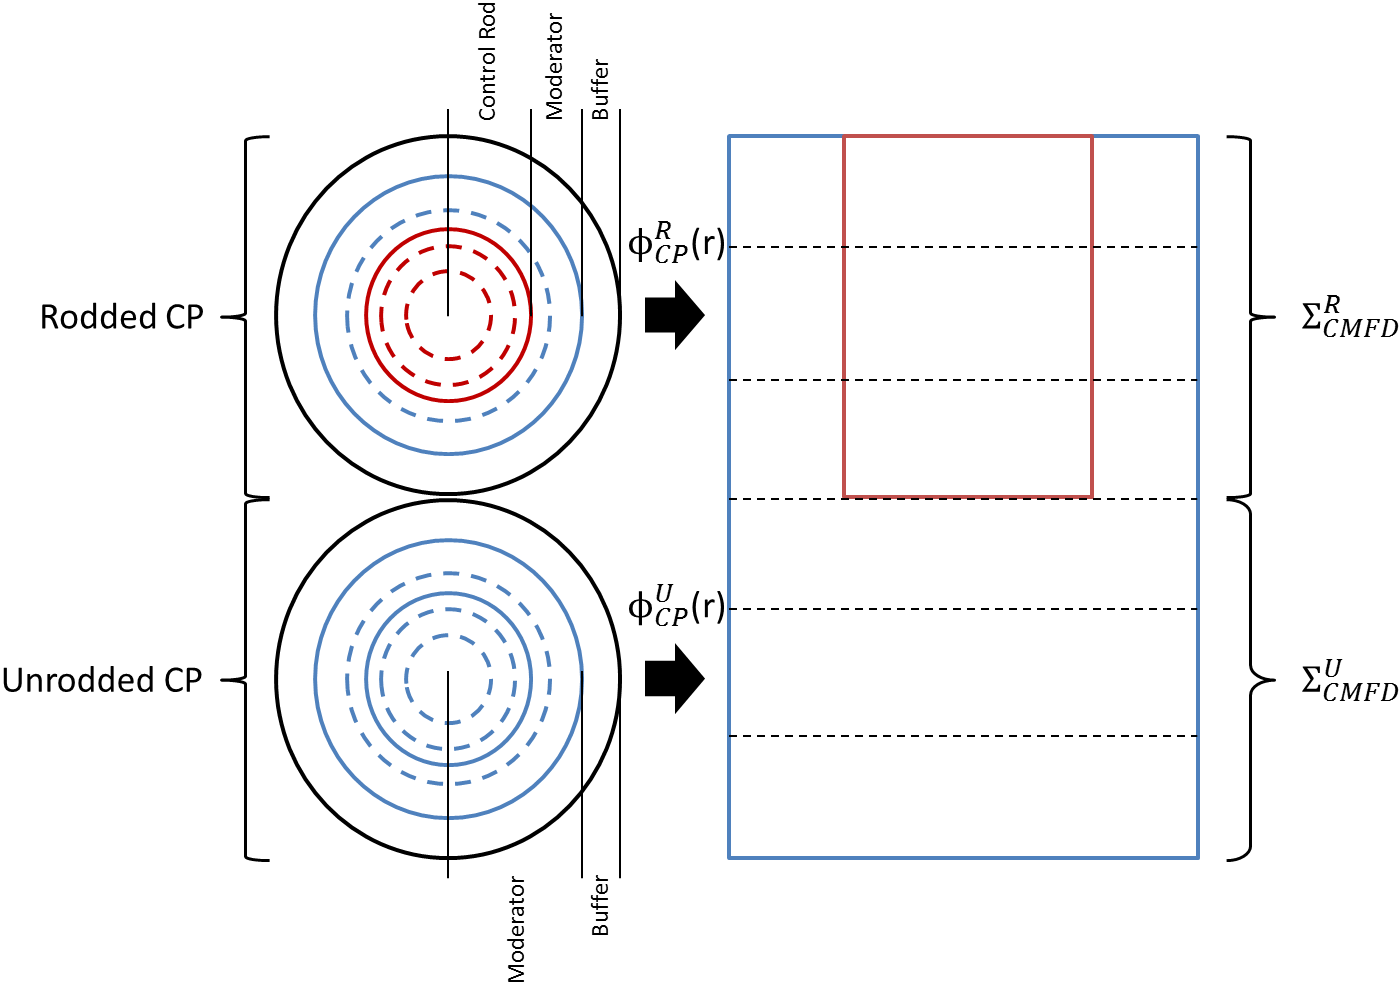
\includegraphics[width=\textwidth]{CPdecusp.png}
    \end{figure}
\end{column}
\end{columns}
    
\end{frame}